\section{Processing methods}
\subsection{Sparsely distributed sensor arrays}
\subsubsection{3D location tracking}
 \begin{figure}[h]
\centering
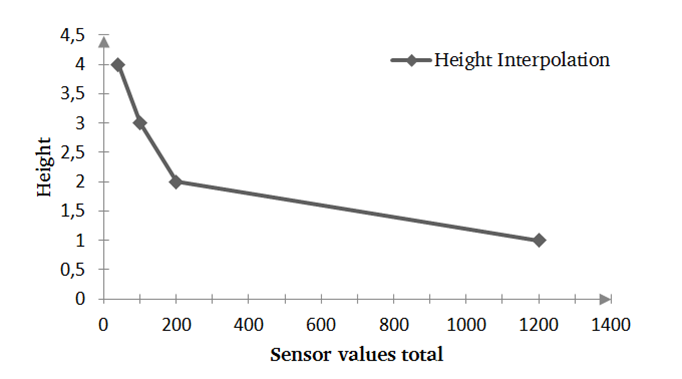
\includegraphics[width=0.6\textwidth]{images/magicbox_data_zaxis}
\caption{Piecewise linear hand distance estimation \cite{Braun2011MultiInputDevice}}
\label{fig:magicbox_data_zaxis}
\end{figure}
%Figure 29 Piecewise linear hand distance estimation [78]
The first data processing step of the MagicBox is the planar localization of the hand, following the weighted average algorithm previously presented. In order to calculate the distance of the hand from the plane we are using a piecewise linear interpolation, that resembles the response curve of a single sensor \cite{Braun2011MultiInputDevice}.
\begin{figure}[h]
\centering
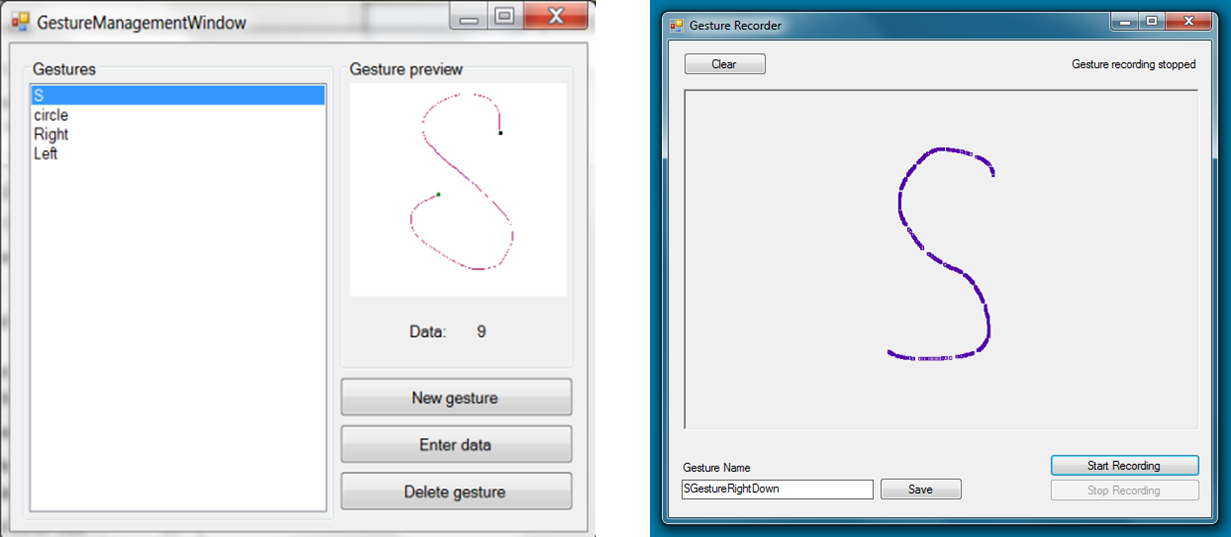
\includegraphics[width=0.7\textwidth]{images/magicbox_data_gest}
\caption{Gesture overview module (left) and gesture recorder (right)}
\label{fig:magicbox_data_gest}
\end{figure}
%Figure 30 Gesture overview module (left) and gesture recorder (right)
An addition of the MagicBox was a generic gesture recognition module based on methods similar to mouse gesture recognition \cite{braun2013capacitive}, albeit adapted for three dimensional locations. The developed debug software allows defining an arbitrary set of potential gestures and adding training data, as shown in Figure \ref{fig:magicbox_data_gest}. The module is looking for matches based on the most recent set of locations. 
\subsubsection{Large-area location tracking}
\subsubsection{Data processing}
Using long wire electrodes may result in considerable noise and influence from outside electric fields. Therefore CapFloor requires preprocessing to reduce the noise and achieve a more robust high-level data processing. The localization uses the weighted average algorithm that has been presented previously. 
\begin{figure}[h]
\centering
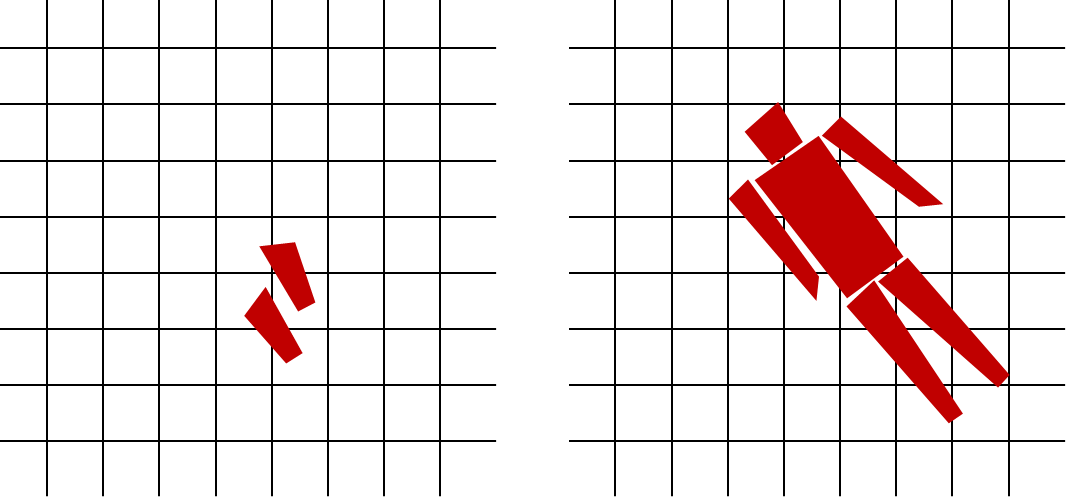
\includegraphics[width=0.8\textwidth]{images/floor_shapes}
\caption{Shapes of a standing and lynig person on top of the CapFloor grid}
\label{fig:capfloor_shapes}
\end{figure}
The fall detection is using a time-series analysis of the aggregated values of the sensors that are currently detecting an object. This method is using the assumption that the overall sensor response is roughly equivalent to the shape of the object that is closest to the surface, resulting in a higher capacitance of the overall system, similar to the plate capacitor model. This effect is shown in Figure \ref{fig:capfloor_shapes}. The sum $s$ of all n sensor values $r$ is the closest equivalent to the system capacitance and therefore a viable measure. If the overall value is beyond a certain threshold $v_l$ we can consider a lying person $p_l$.
\begin{equation}
s=\sum^n_{i=0}{r_i}\ \ \ ,\ \ \ p_l=\left\{ \begin{array}{c}
1,\ \ \ s\ge v_l \\ 
0,\ \ \ s<v_l \end{array}
\right.
\end{equation}
In order to increase the robustness this threshold has to be exceeded for a certain amount of time $t_m$. In consequence a fall $f$ is detected if the following equation is 1.
\begin{equation}
f=\prod^{t_m}_{j=0}{p_{l,t_j}}
\end{equation}
\subsection{Model-driven fitting methods}
\subsubsection{Single-body models}
\begin{figure}[h]
\centering
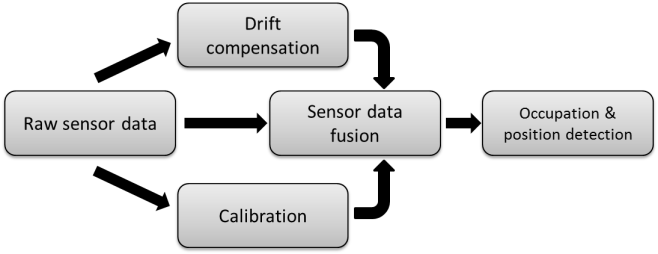
\includegraphics[width=0.7\textwidth]{images/smartbed_proc}
\caption{Data processing components \cite{braun2012context}}
\label{fig:smartbed_proc}
\end{figure}
The different components of the Smart Bed data processing are shown in Figure \ref{fig:smartbed_proc}. Raw sensor data is distributed to three different modules, the calibration which is determining the initial parameters for the sensor data fusion, the drift compensation that alters those parameters according to long term trends and finally the sensor data fusion module that processes the data and does feed it to the occupation \& position detection. Calibration and drift compensation follow the previously presented model \cite{braun2012context}. 
\begin{figure}[h]
\centering
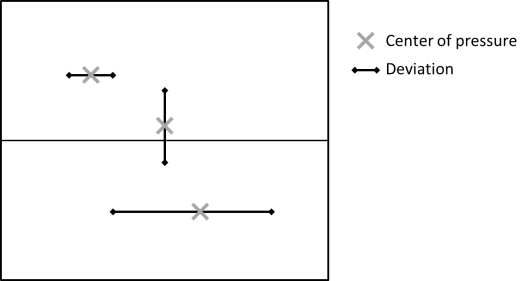
\includegraphics[width=0.7\textwidth]{images/smartbed_cog}
\caption{Calculating centers of pressures and deviation \cite{braun2012context}}
\label{fig:smartbed_cog}
\end{figure}
Occupation and position detection is performed by dividing the two person bed into left and right and individually calculating for each side the total sensor values, assumed center of pressure using weighted average and the standard deviation (Figure \ref{fig:smartbed_cog}). The same calculation is done between the two sides to distinguish where is activity or if one person is lying diagonally.
Using these six intermediate values we can now map various poses. If all activity is on one side and the horizontal deviation is low, we can assume that one person is sitting. We can additionally use the intermediate values to calculate more information, e.g. the exact location a person is sitting at. 
The data processing for the sleep phase recognition is based on detecting the sensor data variations in order to analyze movement. Discriminating between sleep phases using movement is a common approach that has been used in the past \cite{salmi86}. Using a sparse set of sensors it is possible to detect movement by comparing subsequent sensor readings and associate it to different sleep phases using different activity profiles. The system is based on the same prototype as the posture recognition system \cite{Djakow2013movibed}.
\subsubsection{Multi-body models}
\begin{figure}[h]
\centering
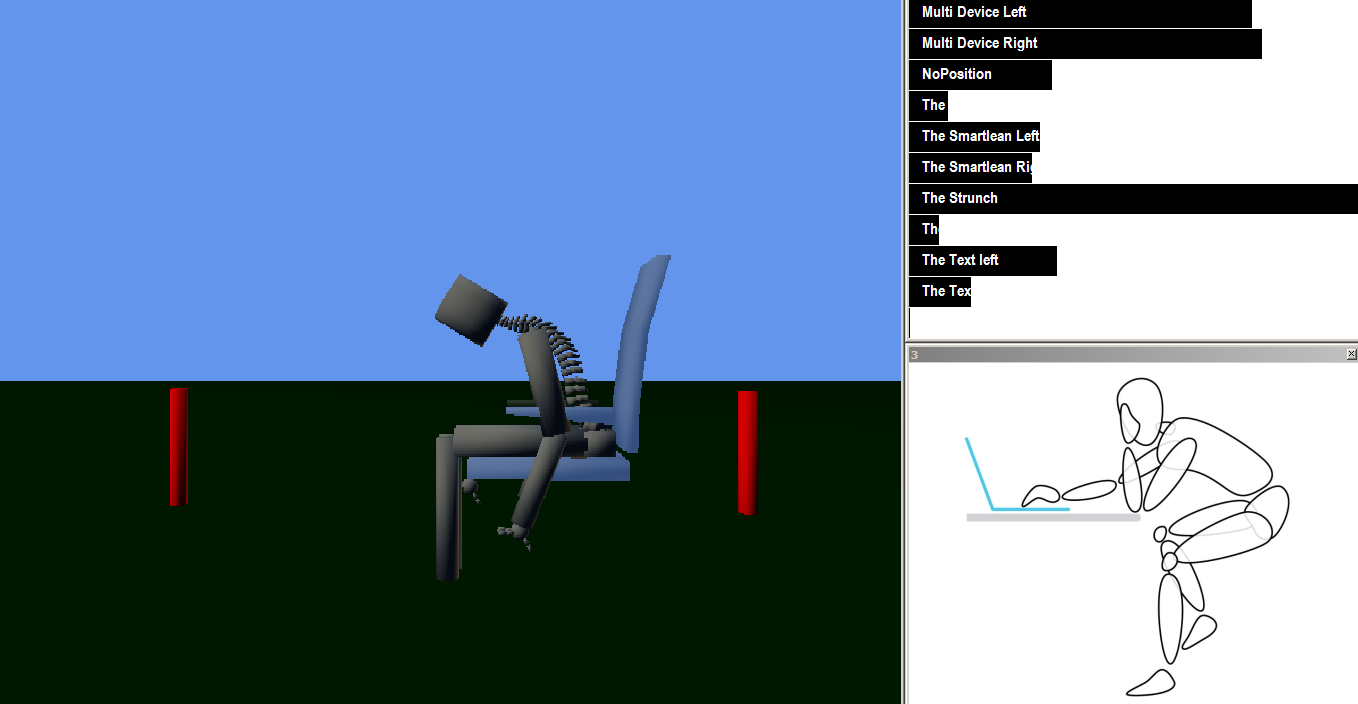
\includegraphics[width=0.7\textwidth]{images/smartchair_software}
\caption{Screenshot of the Capacitive Chair application showing the fitted 3D model on the left, posture detection on the upper right and the recognized posture on the lower right}
\label{fig:smartchair_software}
\end{figure}
In Figure \ref{fig:smartchair_software} we can see a screenshot of the Capacitive Chair debug application. On the left side we see a 3D model that is fitted to a chair model according to the current sensor values, in the middle the results of the machine learning module and the recognized posture and on the right side the currently running breathing rate detection as both Fourier analysis and signal deviation analysis.
All processing methods work on filtered and normalized sensor data. The difference in shape, material and size of the electrodes necessitates slight adaptations to noise filtering and data processing. As an example only the conductive thread backrest electrode is used in the breathing rate detection. 
The 3D model is using a simplified human joint model comprised of 13 connected components. Based on the current sensor readings, single parts or groups of components are fitted to the virtual chair. The process is a mix of posture mapping as found in the smart bed and modification of the dynamic links between the single components \cite{Braun2013ChairAid}.
\begin{figure}[h]
\centering
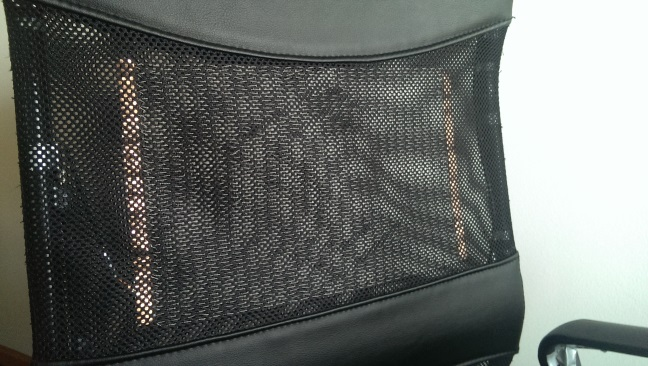
\includegraphics[width=0.7\textwidth]{images/smartchair_thread}
\caption{Screenshot of the Capacitive Chair application showing the fitted 3D model on the left, posture detection on the upper right and the recognized posture on the lower right}
\label{fig:smartchair_thread}
\end{figure}
We use a simple RBF neural network and training data collected by two different persons to match the input from eight sensors to nine potential output postures that are associated to different working situations. An early observation is that certain postures are difficult to distinguish given the limited number of sensors and the similarity of the postures on the rigid chair. Either a higher number of sensors or a more versatile chair could be used that allows gathering additional information required to distinguish the different poses more reliably. 

The breathing rate detection is operating on a single electrode that is integrated into a mesh on the backrest using conductive thread. The setup is shown in Figure \ref{fig:smartchair_thread}. Consequently the surface of the electrode is large and able to pick up the chest movement. Two different methods of data processing are used and fused to get the final breathing rate. Using a fast Fourier transformation the signal is transformed into the frequency space. We are looking for significant signal portions in frequency areas that can be associated to breathing, between $0.2Hz$ and $10Hz$. The second method is to look for zero-crossings of the sensor signal through an adaptive baseline. If a person is breathing in the sensor value will decrease resulting in the signal dropping below the long-term average, and rise above when the person is breathing out. Accordingly the breathing rate can be calculated by counting the zero-crossings.
\subsection{Heterogeneous sensor systems}
\subsubsection{Heterogeneous capacitive arrays}
\begin{figure}[h]
\centering
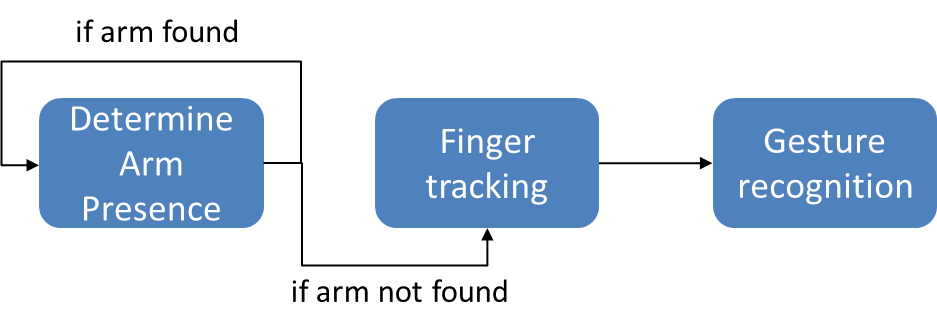
\includegraphics[width=0.4\textwidth]{images/armrest_dataproc}
\caption{Data processing pipeline of Active Armrest}
\label{fig:armrest_dataproc}
\end{figure}
%Figure 25 Data processing pipeline of Active Armrest
As we already mentioned, the Active Armrest electrodes are put into two groups. The data processing for both groups is distinctly different. In order to detect the presence of the arm using the two-electrode group a simple threshold on the accumulated values is used. The six sensor array in the front (touch area) is using the presented weighted average method to calculate finger positions. Additionally a threshold is used to distinguish one and two fingers. Overall there is a data processing pipeline as shown in Figure \ref{fig:armrest_proto}. The finger tracking and gesture recognition will be inactive until it is ensured that no arm is present. 
\subsubsection{Evaluation}
\begin{figure}[h]
\centering
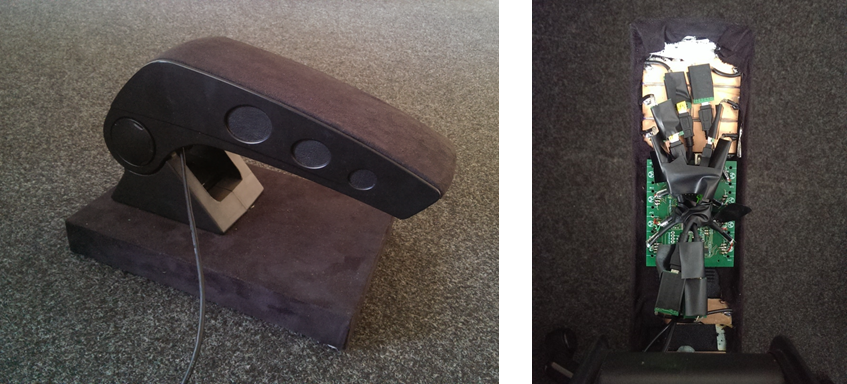
\includegraphics[width=0.8\textwidth]{images/armrest_proto}
\caption{Active Armrest prototype, left - outside view, right - detail view of electronics}
\label{fig:armrest_proto}
\end{figure}
%Figure 26 Active Armrest prototype, left - outside view, right - detail view of electronics
In order to evaluate the Active Armrest we have built the prototype shown in Figure \ref{fig:armrest_dataproc}. An aftermarket armrest was equipped with an OpenCapSense toolkit. The demonstration application is based on the SenseKit debug software supplied with the toolkit. As of now there is a simple USB connection to a nearby PC.
\begin{figure}[h]
\centering
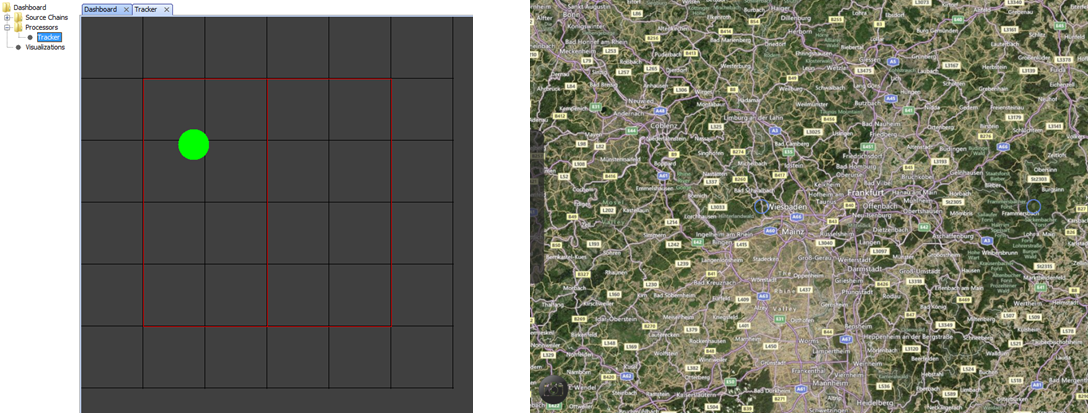
\includegraphics[width=0.6\textwidth]{images/armrest_eval}
\caption{Active Armrest demo software, left - finger tracker, right - OSM based navigation application}
\label{fig:armrest_eval}
\end{figure}
%Figure 27 Active Armrest demo software, left - finger tracker, right - OSM based navigation application
Figure \ref{fig:armrest_eval} shows a screenshot of the finger tracking application on the left, with a two-finger touch registered on the upper left part of the touch area. It is interfaced with a TUIO \cite{kaltenbrunner2005tuio} based maps application using OpenStreetMap \cite{haklay2008openstreetmap} data. The map is moved around using simple swipe movements of the finger that are directly associated to pan-features of the demonstration application. Zooming is activated by two-finger hold gestures on the upper or lower part of the touch area. We have used public displays of this prototype to get an idea of how easily unaffiliated persons learn to use the system. While the majority agreed on the potential of the application, there have been some reservations regarding the current gesture set, particularly that a closer relationship to smartphone touch screen gestures would be welcome.
\subsubsection{Heterogeneous sensor fusion}
\begin{figure}[h]
\centering
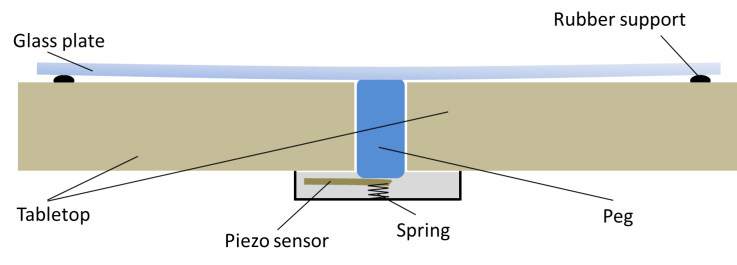
\includegraphics[width=0.7\textwidth]{images/captap_peg}
\caption{Suspended peg knock detection system for CapTap \cite{Braun2013ChairAid}}
\label{fig:captap_peg}
\end{figure}
%Figure 34 Suspended peg knock detection system for CapTap [80]
The hand location of the CapTap is similar to the methods presented for the MagicBox. We add the additional component of knock detection to provide selection events when touching the surface. Figure \ref{fig:captap_sketch} shows a sketch of the knock detection system. The table has a glass plate that is suspended on some rubber supports. In the center of the table we attach a small peg (enlarged in sketch) that creates a connection between the glass plate and a piezo sensor. If the glass plate starts vibrating from a touch we can measure this using the piezo sensor \cite{Braun2013ChairAid}. If a notable vibration is measured we are collecting the next 50 samples, resulting in a window of 250 milliseconds. To distinguish single and double knocks we calculate the weighted average within this window to get a measure for the distribution of sensor values within. If the average is closer to the beginning of the window the resulting event should be a single knock, and a double if the average is closer to the end of the window.
Hand localization and knock detection are working independently and are combined later in the software. It is reasonable to combine this, e.g. to ignore knock events that are occurring without a hand present. They may be indicative of a person doing a strong step close to the table.
\subsubsection{Evaluation}
\begin{figure}[h]
\centering
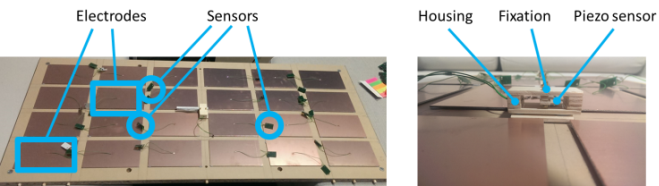
\includegraphics[width=0.7\textwidth]{images/captap_proto}
\caption{Detail views of the prototype system: left - electrode and sensors, right - knock detection box \cite{Braun2013ChairAid}}
\label{fig:captap_proto}
\end{figure}
%Figure 35 Detail views of the prototype system: left - electrode and sensors, right - knock detection box [80]
The CapTap prototype is integrated into a common living room table. Some photos can be seen in Figure \ref{fig:captap_proto}. On the left side we see the 24 electrodes made of non-etched circuit boards. A sensor is attached to each. The knock detection box with fixation, housing and piezo sensor is shown on the right side.
\begin{figure}[h]
\centering
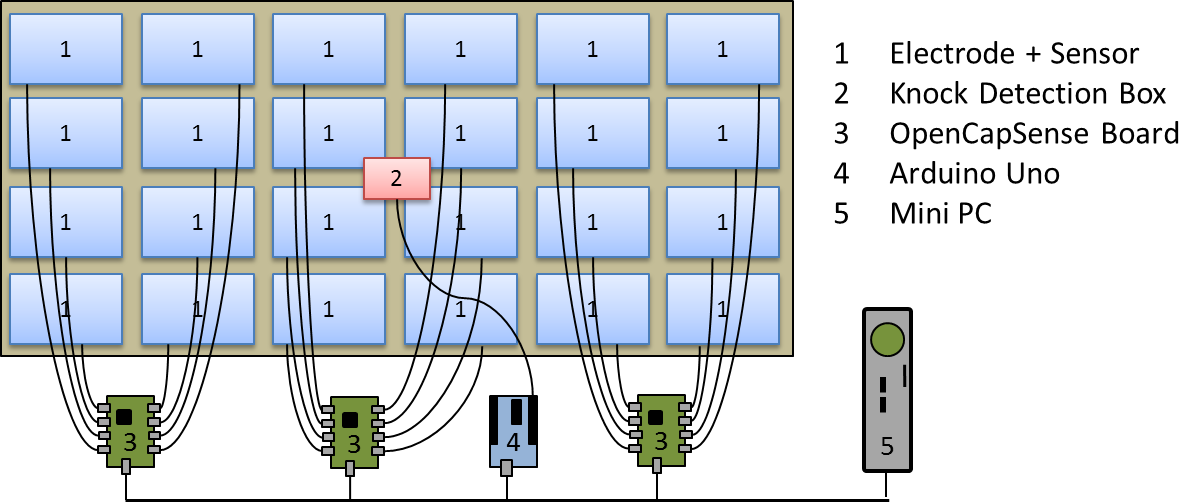
\includegraphics[width=0.7\textwidth]{images/captap_system}
\caption{Abstracted view of CapTap prototype including capacitive sensing electrodes and knock detection sensor \cite{Braun2013ChairAid}}
\label{fig:captap_system}
\end{figure} 
%Figure 36 Abstracted view of CapTap prototype including capacitive sensing electrodes and knock detection sensor [80]
The overall abstracted layout of the prototype is shown in Figure \ref{fig:captap_system}. The capacitive sensors are con-trolled by three OpenCapSense boards; the knock detection is performed on an Arduino Uno microcontroller board. The data fusion is outsourced to a Mini-PC that can be placed in the table.
Various evaluations have been performed with the CapTap. We have benchmarked the hand localization against the Leap Motion, concluding that the algorithm works reasonably precise in most parts of the interaction area. The next study was a quantitative study of the percentage of correctly recognized knocks, resulting in considerable misattribution of single and double knocks, due to strongly varying knocking styles. However, the presence of any knock was detected with a precision of about $90\%$ \cite{Braun2013ChairAid}. Our main evaluation of the system was concerned with the influence of our knock detection on the overall interaction speed of the system. The results concluded that merely adding the knock detection is not enough but that additionally the interfaces have to be adapted towards capacitive systems \cite{Braun2013ChairAid}.

\subsection{Image-based processing}
